\documentclass{beamer}

\usepackage{ulem}
\usepackage{amsmath}
\usepackage{mathdots}
\pagenumbering{arabic}
\usepackage{hyperref}
\usepackage{lscape}
\definecolor{slidetitlecolor}{RGB}{51,0,102}
\usenavigationsymbolstemplate{}
\setbeamertemplate{footline}[frame number]%puts frame numbers in slide
\setbeamercolor{frametitle}{fg=slidetitlecolor}
\definecolor{item1color}{RGB}{51,153,255}
\setbeamercolor{itemize item}{fg=item1color}
\setbeamertemplate{itemize item}[circle]
\setbeamercolor{enumerate item}{fg=item1color}

\title{Game Theory\vspace{-.5cm}}
\author{VK\\
Room: M1.30\\
\url{knightva@cf.ac.uk}\\
\url{www.vincent-knight.com}\\}
\date{\tiny{Last updated: \today.}}





\begin{document}

\maketitle


\frame{\frametitle{Overview}\tableofcontents}
\section{Normal Form Games}
\frame{\frametitle{Normal Form Games}}
\frame{\frametitle{Game Theory: Introduction}
Often decision analysis does not only depend on chance but on the decisions made by others: \emph{interactive decision problems}.\\\vspace{.5cm}
Such decision problems are called \emph{games}. The individuals making the decisions are called \emph{players}.}

\frame{\frametitle{2 Player Static Games}}
\frame{\frametitle{2 Player Static Games}
We shall consider 2 player static games. Assume two players have two sets of available strategies: $S_1=\{r_1,\dots,r_m\}$ and $S_2=\{s_1,\dots,s_n\}$. Let $u_1(r,s),\; u_2(r,s)$ be the utility gained by player 1 and 2 for a pair of strategies $(s,r)$. \pause
$$\begin{tabular}{|c|c|c|c|c|}
\hline
 &$s_1$      &$s_2$   &\dots&$s_n$  \\\hline
$r_1$&$(u_1,u_2)$&$(u_1,u_2)$&\dots&$(u_1,u_2)$\\\hline
$r_2$&$(u_1,u_2)$&$(u_1,u_2)$&\dots&$(u_1,u_2)$\\\hline
$\vdots$&$\vdots$&$\vdots$&$\ddots$&$\vdots$\\\hline
$r_m$&$(u_1,u_2)$&$(u_1,u_2)$&\dots&$(u_1,u_2)$\\\hline
\end{tabular}$$\pause
Both players aim to choose from their available strategies so as to maximise $u_1$ and $u_2$.
}

\frame{\frametitle{Example: Prisoner's Dilemma}
Two criminal suspects have been caught. They have been isolated and are being questioned separately by the police. The following offer is made to both suspects:
\begin{itemize}
\item If one confesses that they both committed the crime then the confessor will be set free and the other will spend 5 years in jail.
\item If both confess, then they will each get a 4 year sentence.
\item If neither confess, then they will each spend 2 years in jail.
\end{itemize}
}

\frame{\frametitle{Example: Prisoner's Dilemma}
Both \emph{players} have 2 possible strategies:\begin{itemize}
\item Keep quite (Q)
\item Squeal (S)
\end{itemize}
\pause


%\psgrid(3,0)(7,5)
$$\begin{tabular}{|c|c|c|}
\hline
 &$Q$      &$S$     \\\hline
$Q$&(-2,-2)&(-5,0)\\\hline
$S$&(0,-5)&(-4,-4)\\\hline
\end{tabular}$$\pause

The ``solution'' of the game is $(S,S)$. Both criminals squeal and go to prison for 4 years (Instead of 2).

}

\frame{\frametitle{Solving games using Dominance}
We solved the prisoners' dilemma in an intuitively simple manner by observing the strategy $S$ was always ``better'' then $Q$. We attempt to solve games by eliminating poor strategies for each player.\\\vspace{.5cm}
\begin{itemize}\item A strategy for player 1, $r_i$ is, \emph{strictly dominated} by $r_j$ if
$$u_1(r_i,s)< u_1(r_j,s) \text{ for all }s\in S_2$$
\item A strategy for player 1, $r_i$ is, \emph{weakly dominated} by $r_j$ if
$$u_1(r_i,s)\leq u_1(r_j,s) \text{ for all }s\in S_2$$
and there exists a strategy $s_l\in S_2$ such that:
$$u_1(r_i,s_l)< u_1(r_j,s_l)$$
\end{itemize}}

\frame{\frametitle{Example}
Consider the following game:
\begin{center}$\begin{tabular}{|c|c|c|}
\hline
 &$s_1$      &$s_2$     \\\hline
$r_1$&$(3,3)$&$(2,2)$\\\hline
$r_2$&$(2,1)$&$(2,1)$\\\hline
\end{tabular}$
\end{center}


For player 2, $s_1$ weakly dominates $s_2$. For player 1, $r_1$ weakly dominates $r_2$. Thus $(r_1,s_1)$ is the ``solution'' of this game.
}

\frame{\frametitle{Common Knowledge of Rationality}
To solve a game by elimination of dominated strategies we have to assume that the players are rational. However, we can go further, if we also assume that:
\begin{itemize}
\item The players are rational.\pause
\item The players all know that the other players are rational.\pause
\item The players all know that the other players know that they are rational.\pause
\item \dots
\end{itemize}
This chain of assumptions is called \emph{Common Knowledge of Rationality} (CKR). By applying the CKR assumption, we can try to solve games by iterating the elimination of dominated strategies.}

\frame{\frametitle{Example}
$$\begin{tabular}{|c|c|c|c|}
\hline
 &$s_1$      &$s_2$  &$s_3$   \\\hline
$r_1$&$(1,0)$&$(1,2)$&$(0,1)$\\\hline
$r_2$&$(0,3)$&$(0,1)$&$(2,0)$\\\hline
\end{tabular}$$
\textbf{Initially} player 1 has no dominated strategies. For player 2, $s_3$ is dominated by $s_2$. \textbf{Now}, $r_2$ is dominated by $r_1$. \textbf{Finally}, $s_1$ is dominated by $s_2$. Thus $(r_1,s_2)$ is the ``solution'' of this game.
}

\section{Pure Nash Equilibrium}
\frame{\frametitle{Pure Nash Equilibrium}}
\frame{\frametitle{(Pure) Nash Equilibrium}
Importantly, certain games cannot be solved using the iterated elimination of dominated strategies:
$$\begin{array}{c@{\hspace{1cm}}c}
\begin{tabular}{|c|c|c|c|}
\hline
 &$s_1$      &$s_2$  &$s_3$   \\\hline
$r_1$&$(10,0)$&$(5,1)$&$(4,-2)$\\\hline
$r_2$&$(10,1)$&$(5,0)$&$(1,-1)$\\\hline
\end{tabular}
&
\begin{tabular}{|c|c|c|c|}
\hline
 &$s_1$      &$s_2$  &$s_3$   \\\hline
$r_1$&$(1,3)$&$(4,2)$&$(2,2)$\\\hline
$r_2$&$(4,0)$&$(0,3)$&$(4,1)$\\\hline
$r_3$&$(2,5)$&$(3,4)$&$(5,6)$\\\hline
\end{tabular}
\end{array}$$\pause
(exercise: why does iterated elimination fail here?)
}

\frame{\frametitle{Nash Equilibrium}
A (pure) \emph{Nash equilibrium} is a pair of strategies $(\tilde r,\tilde s)$ such that
$$u_1(\tilde r,\tilde s)\geq u_1(r,\tilde s)\text{ for all }r\in S_1$$
and
$$u_2(\tilde r,\tilde s)\geq u_2(\tilde r, s)\text{ for all }s\in S_2$$}

\frame{\frametitle{Testing for Nash Equilibrium}
One can find Nash equilibria by checking all strategy pairs and seeing if either player can improve their outcome.
\begin{center}\begin{tabular}{|c|c|c|c|}
\hline
 &$s_1$      &$s_2$  &$s_3$   \\\hline
$r_1$&$(10,0)$&$(5,1)$&$(4,-2)$\\\hline
$r_2$&$(10,1)$&$(5,0)$&$(1,-1)$\\\hline
\end{tabular}
\end{center}
\pause
Nash Equilibria need not be unique!
}

\frame{\frametitle{Best response strategies}
A strategy for player 1 $r^*$ is a \emph{best response }to some fixed strategy for player 2, $s$ if:
$$u_1(r^*,s)\geq u_1(r,s)\text{ for all }r\in S_1$$
A strategy for player 2 $s^*$ is a \emph{best response }to some fixed strategy for player 1, $r$ if:
$$u_2(r,s^*)\geq u_2(r,s)\text{ for all }s\in S_2$$\pause
To use this definition to find Nash Equilibria we find for each player, the set of best responses to every possible strategy of the other player. We then look for pairs of strategies that are best responses to each other.
}




\frame{\frametitle{Example}
\begin{center}
\begin{tabular}{|c|c|c|c|}
\hline
 &$s_1$      &$s_2$  &$s_3$   \\\hline
$r_1$&$(1,3)$&$(4,2)$&$(2,2)$\\\hline
$r_2$&$(4,0)$&$(0,3)$&$(4,1)$\\\hline
$r_3$&$(2,5)$&$(3,4)$&$(5,6)$\\\hline
\end{tabular}
\end{center}
}


\section{Mixed Nash Equilibrium}
\frame{\frametitle{Mixed Nash Equilibrium}}


\frame{\frametitle{Mixed Strategies}
Importantly some games do not have \textbf{pure} Nash equilibria! Consider the following game:\\\vspace{.5cm}
Two players each place a coin on a table, either ``heads up'' (strategy $H$) or ``tails up'' (strategy $T$). If the pennies match, player 1 wins, if the pennies differ, then player 2 wins.\pause
\begin{center}
\begin{tabular}{|c|c|c|}
\hline
 &$H$      &$T$     \\\hline
$H$&$(1,-1)$&$(-1,1)$\\\hline
$T$&$(-1,1)$&$(1,-1)$\\\hline
\end{tabular}
\end{center}
}

\frame{\frametitle{Mixed Strategies}
In order to solve such games, we need to consider \emph{mixed strategies}. I.e. we attach a distribution to the set of strategies of each player.\\\vspace{.5cm} In the \emph{matching pennies} example, let $\rho=(p,1-p)$ be the mixed strategy for player 1. I.e. player 1 plays $H$ with probability $p$ and plays $T$ with probability $1-p$.\\\vspace{.5cm} Similarly let $\sigma=(q,1-q)$ be the mixed strategy for player 2. I.e. player 2 plays $H$ with probability $q$ and plays $T$ with probability $1-q$.
}

\frame{\frametitle{Mixed Strategies}
Consider the payoff to player 1:
$$
\begin{array}{@{}r@{\;}c@{\;}l@{}}
u_1(\rho,\sigma)&=&pq-p(1-q)-(1-p)q+(1-p)(1-q)\\[2mm]
                &=&1-2q+2p(2q-1)\\[2mm]
                &=&(2q-1)(2p-1)
\end{array}
$$
\begin{itemize}
\item If $q<{1\over2}$ then player 1s best response is to choose $p=0$ (i.e. always play $T$).
\item If $q>{1\over2}$ then player 1s best response is to choose $p=1$ (i.e. always play $H$).
\item If $q={1\over2}$ then player 1s best response is to play any mixed strategy.
\end{itemize}
}

\frame{\frametitle{Mixed Strategies}
Consider the payoff to player 2:
$$
\begin{array}{@{}r@{\;}c@{\;}l@{}}
u_2(\rho,\sigma)&=&-pq+p(1-q)+(1-p)q-(1-p)(1-q)\\[2mm]
                &=&-1+2q-2p(2q-1)\\[2mm]
                &=&(2q-1)(1-2p)
\end{array}
$$
\begin{itemize}
\item If $p<{1\over2}$ then player 2s best response is to choose $q=1$ (i.e. always play $H$).
\item If $p>{1\over2}$ then player 2s best response is to choose $q=0$ (i.e. always play $T$).
\item If $p={1\over2}$ then player 2s best response is to play any mixed strategy.
\end{itemize}
}

\frame{\frametitle{Mixed Strategies}
The only pair of strategies that are best responses to each other is $\rho=\sigma=\left({1\over2},{1\over2}\right)$.\\\vspace{.5 cm}

This method of finding mixed Nash equilibria is called: the \emph{best response} method. (Of course it also finds the pure Nash equilibria)
\\\vspace{.5 cm}
Exercise: Do the same exercise for the popular game ``rock,paper scissors''.
}

\frame{\frametitle{Example}
\begin{center}
\begin{tabular}{|c|c|c|}
\hline
 &$s_1$      &$s_2$     \\\hline
$r_1$&$(0,0)$&$(2,1)$\\\hline
$r_2$&$(1,2)$&$(0,0)$\\\hline
\end{tabular}
\end{center}\pause As before:
$$\begin{array}{@{}r@{\;}c@{\;}l@{}}
u_1(\rho,\sigma)&=&q+p(2-3q)\\
u_2(\rho,\sigma)&=&p+q(2-3p)\\
\end{array}
$$\pause
Best responses for player 1:
$$
\rho^*=\left\{\;\begin{array}{@{}l@{\;}r@{}}
(0,1)&\text{ if }q>{2\over3}\\[2mm]
(1,0)&\text{ if }q<{2\over3}\\[2mm]
(x,1-x)\text{ with }0\leq x\leq1&\text{ if }q={2\over3}\\[2mm]
\end{array}\right.
$$
}

\frame{\frametitle{Example}
\begin{center}
\begin{tabular}{|c|c|c|}
\hline
 &$s_1$      &$s_2$     \\\hline
$r_1$&$(0,0)$&$(2,1)$\\\hline
$r_2$&$(1,2)$&$(0,0)$\\\hline
\end{tabular}
\end{center} As before:
$$\begin{array}{@{}r@{\;}c@{\;}l@{}}
u_1(\rho,\sigma)&=&q+p(2-3q)\\
u_2(\rho,\sigma)&=&p+q(2-3p)\\
\end{array}
$$
Best responses for player 2:
$$
\sigma^*=\left\{\;\begin{array}{@{}l@{\;}r@{}}
(0,1)&\text{ if }p>{2\over3}\\[2mm]
(1,0)&\text{ if }p<{2\over3}\\[2mm]
(y,1-y)\text{ with }0\leq y\leq1&\text{ if }p={2\over3}\\[2mm]
\end{array}\right.
$$
}

\frame{\frametitle{Example}
We plot both best responses:
\begin{center}
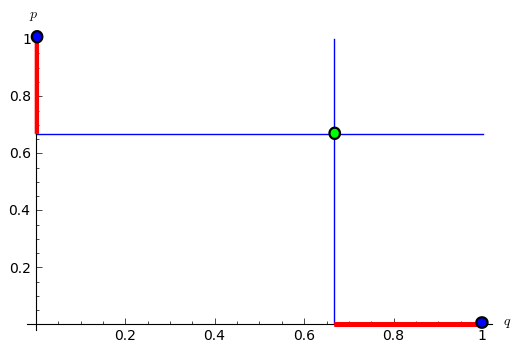
\includegraphics[width=10cm]{Best_Responses}
\end{center}
}

\frame{\frametitle{Example}
Thus for this example there are 3 Nash equilibria:
$$(r_1,s_2),\;(r_2,s_1)\text{ and }(\rho,\sigma)\text{ with }\rho=\sigma=\left({2\over3},{1\over3}\right)$$
}

\frame{\frametitle{Equality of Payoffs}
The \emph{support} of a strategy $\rho$ is the set $S(\rho)$ of all strategies for which $\rho$ has non zero probability.\\\vspace{.5cm}
For example, if the strategy set is $\{A,B,C\}$ then the support of the mixed strategy $\left({1\over3},{2\over3},0\right)$ is $\{A,B\}$. Similarly the support of the mixed strategy $\left({1\over2},0,{1\over2}\right)$ is $\{A,C\}$.\\\vspace{.5cm}
This leads to a very powerful result.
}

\frame{\frametitle{Equality of Payoffs Theorem}
Let $(\rho,\sigma)$ be a Nash equilibrium, and let $S_1^*$ be the support of $\rho$. Then:
$$u_1(\rho,\sigma)=u_1(r,\sigma)\text{ for all }r\in S_1^*$$
}

\frame{\frametitle{Equality of Payoffs}
Consider the \emph{matching pennies} game. Let $\sigma$ be the mixed strategy of player 2 with a chance of playing $H$ of $q$ and a chance of playing $T$ with probability $(1-q)$. From the Equality of Payoffs theorem we have:
$$\begin{array}
{c}u_1(H,\sigma)=u_1(T,\sigma)\\[2mm]
qu_1(H,H)+(1-q)u_1(H,T)=qu_1(T,H)+(1-q)u_1(T,T)\\[2mm]
q-(1-q)=-q+(1-q)\\[2mm]
q={1\over2}
\end{array}$$
}

\frame{\frametitle{Equality of Payoffs}
Let $\rho$ be the mixed strategy of player 1 with a chance of playing $H$ of $p$ and a chance of playing $T$ with probability $1-p$.From the Equality of Payoffs theorem we also have:
$$\begin{array}
{c}u_2(\rho,H)=u_2(\rho,T)\\[2mm]
pu_2(H,H)+(1-p)u_2(T,H)=pu_2(H,T)+(1-p)u_2(T,T)\\[2mm]
-p+(1-p)=p-(1-p)\\[2mm]
p={1\over2}
\end{array}$$
As expected.
}

\frame{\frametitle{Nash's Theorem}
\it{Every game that has a finite set of strategies has at least one Nash equilibrium (involving pure or mixed strategies).}\\\vspace{.5cm}
(It can be shown that there is always an odd number of Nash equilibria.)
}


\end{document}
